
\subsection{\texttt{un-semun-frontend}: A React \& Sigma.js frontend} \label{ssec:un-semun-frontend-a-react-sigma-js-frontend}

I used React combined with Typescript for the UI framework, as well as \href{https://chakra-ui.com/}{Chakra UI} for the UI components and \href{https://www.sigmajs.org/}{\texttt{Sigma.js}}, via its React adapter \href{https://sim51.github.io/react-sigma/}{\texttt{@react-sigma}} for the network map. \href{https://graphology.github.io/}{\texttt{graphology}} was also used for graph manipulation in the frontend, mostly to iterate over graph elements to perform styling. The code is available here: \repo{un-semun-frontend}.


\begin{figure}[!htb]
    \centering

    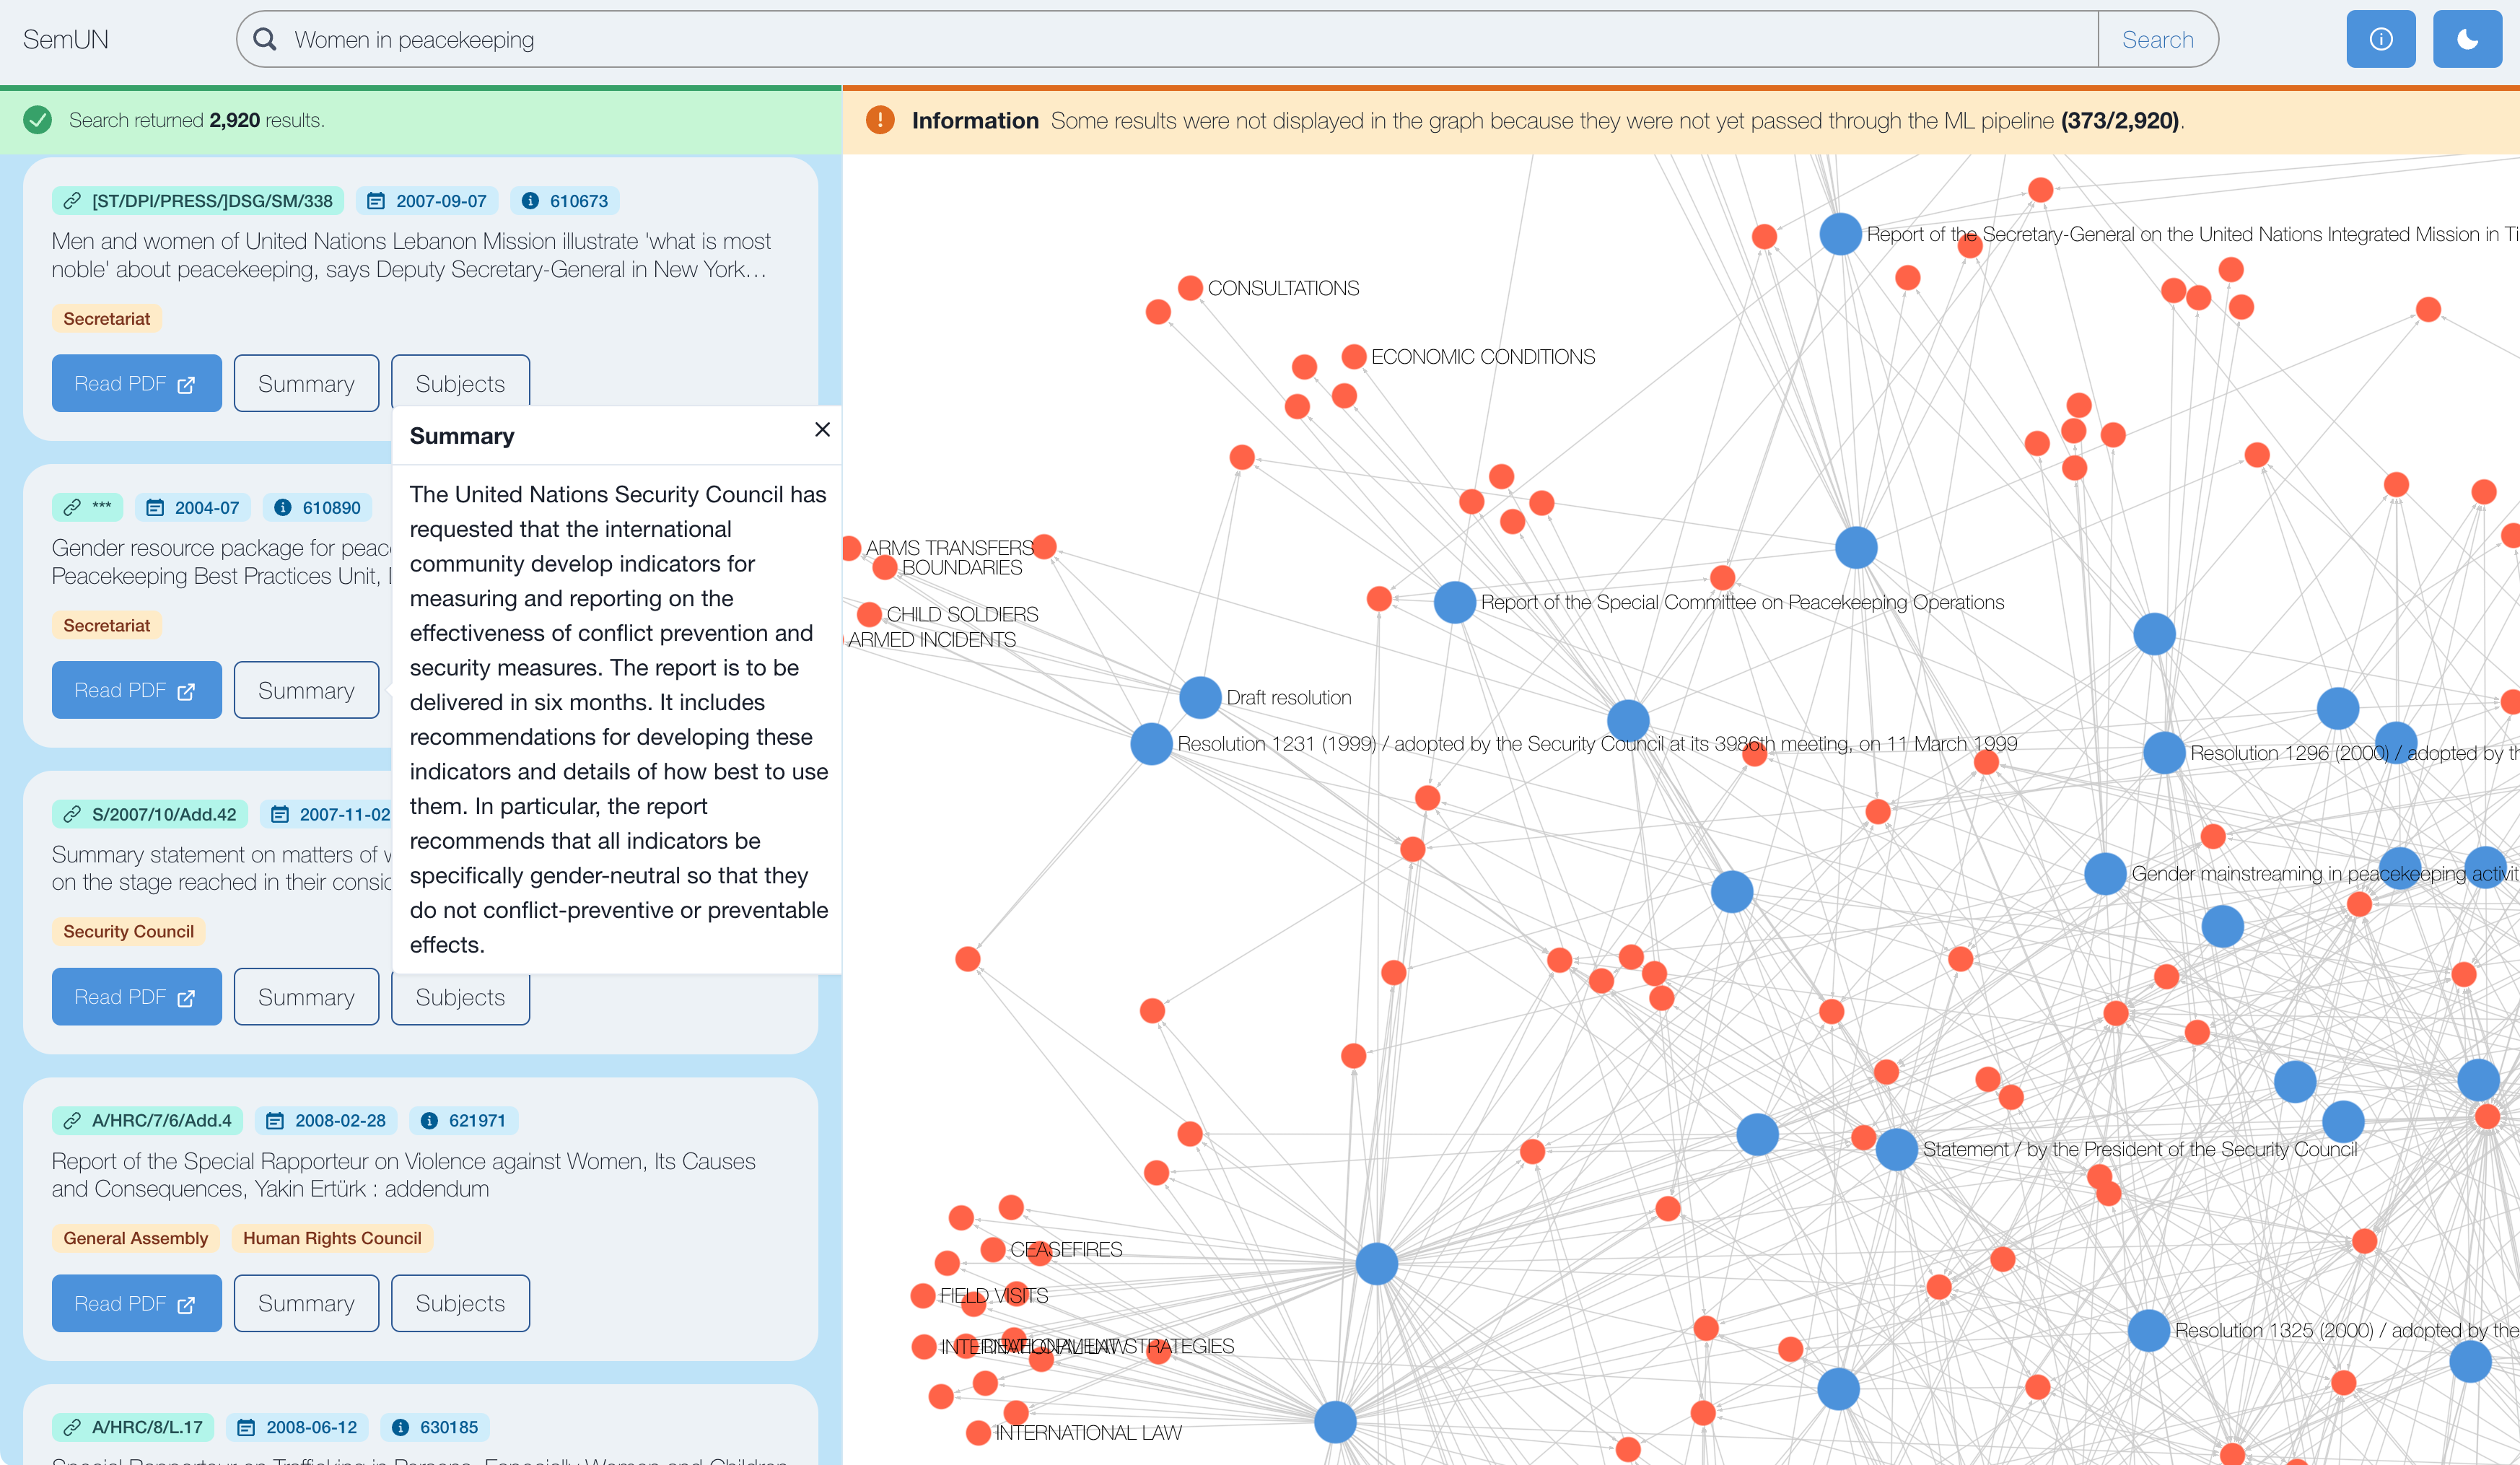
\includegraphics[width=\linewidth]{res/un-frontend.png}
    \caption{Screenshot of the frontend on the query \texttt{"Women in peacekeeping"}.}
    % change caption position to the bottom

    \label{fig:frontend-screenshot}
\end{figure}


The frontend was the part I was the least familiar with, but Chakra UI allowed to insert nice-looking components that I could customize based on my use case. It is composed in two panes:

\begin{itemize}
    \item \textbf{The search bar} (on top): the user can enter its prompt, which will be sent to the API (\ref{ssec:un-semun-api-an-api-for-un-semun-frontend-using-fastapi}) to retrieve the results.
    \item \textbf{The result list} (on the left). The results are displayed as a scrollable list of \texttt{Card} components, with the title, the summary, and the date of publication. The user can click on a card to display the document in the right pane.
    \item \textbf{The network map} (on the right). The results of the search are also displayed as a network map, with the documents, related United Nations bodies, topics from UNBIS Thesaurus taxonomy, and named entities extracted from the documents. The user can click on a node to display the document in the left pane. This map is also fetched using the API (\ref{ssec:un-semun-api-an-api-for-un-semun-frontend-using-fastapi}) and is based on the results of the machine learning pipeline (\ref{ssec:un-ml-pipeline-the-machine-learning-pipeline}).
\end{itemize}

